\usetikzlibrary{mindmap,backgrounds,shapes.misc}

\begin{center}
\resizebox{0.9\textwidth}{!}{
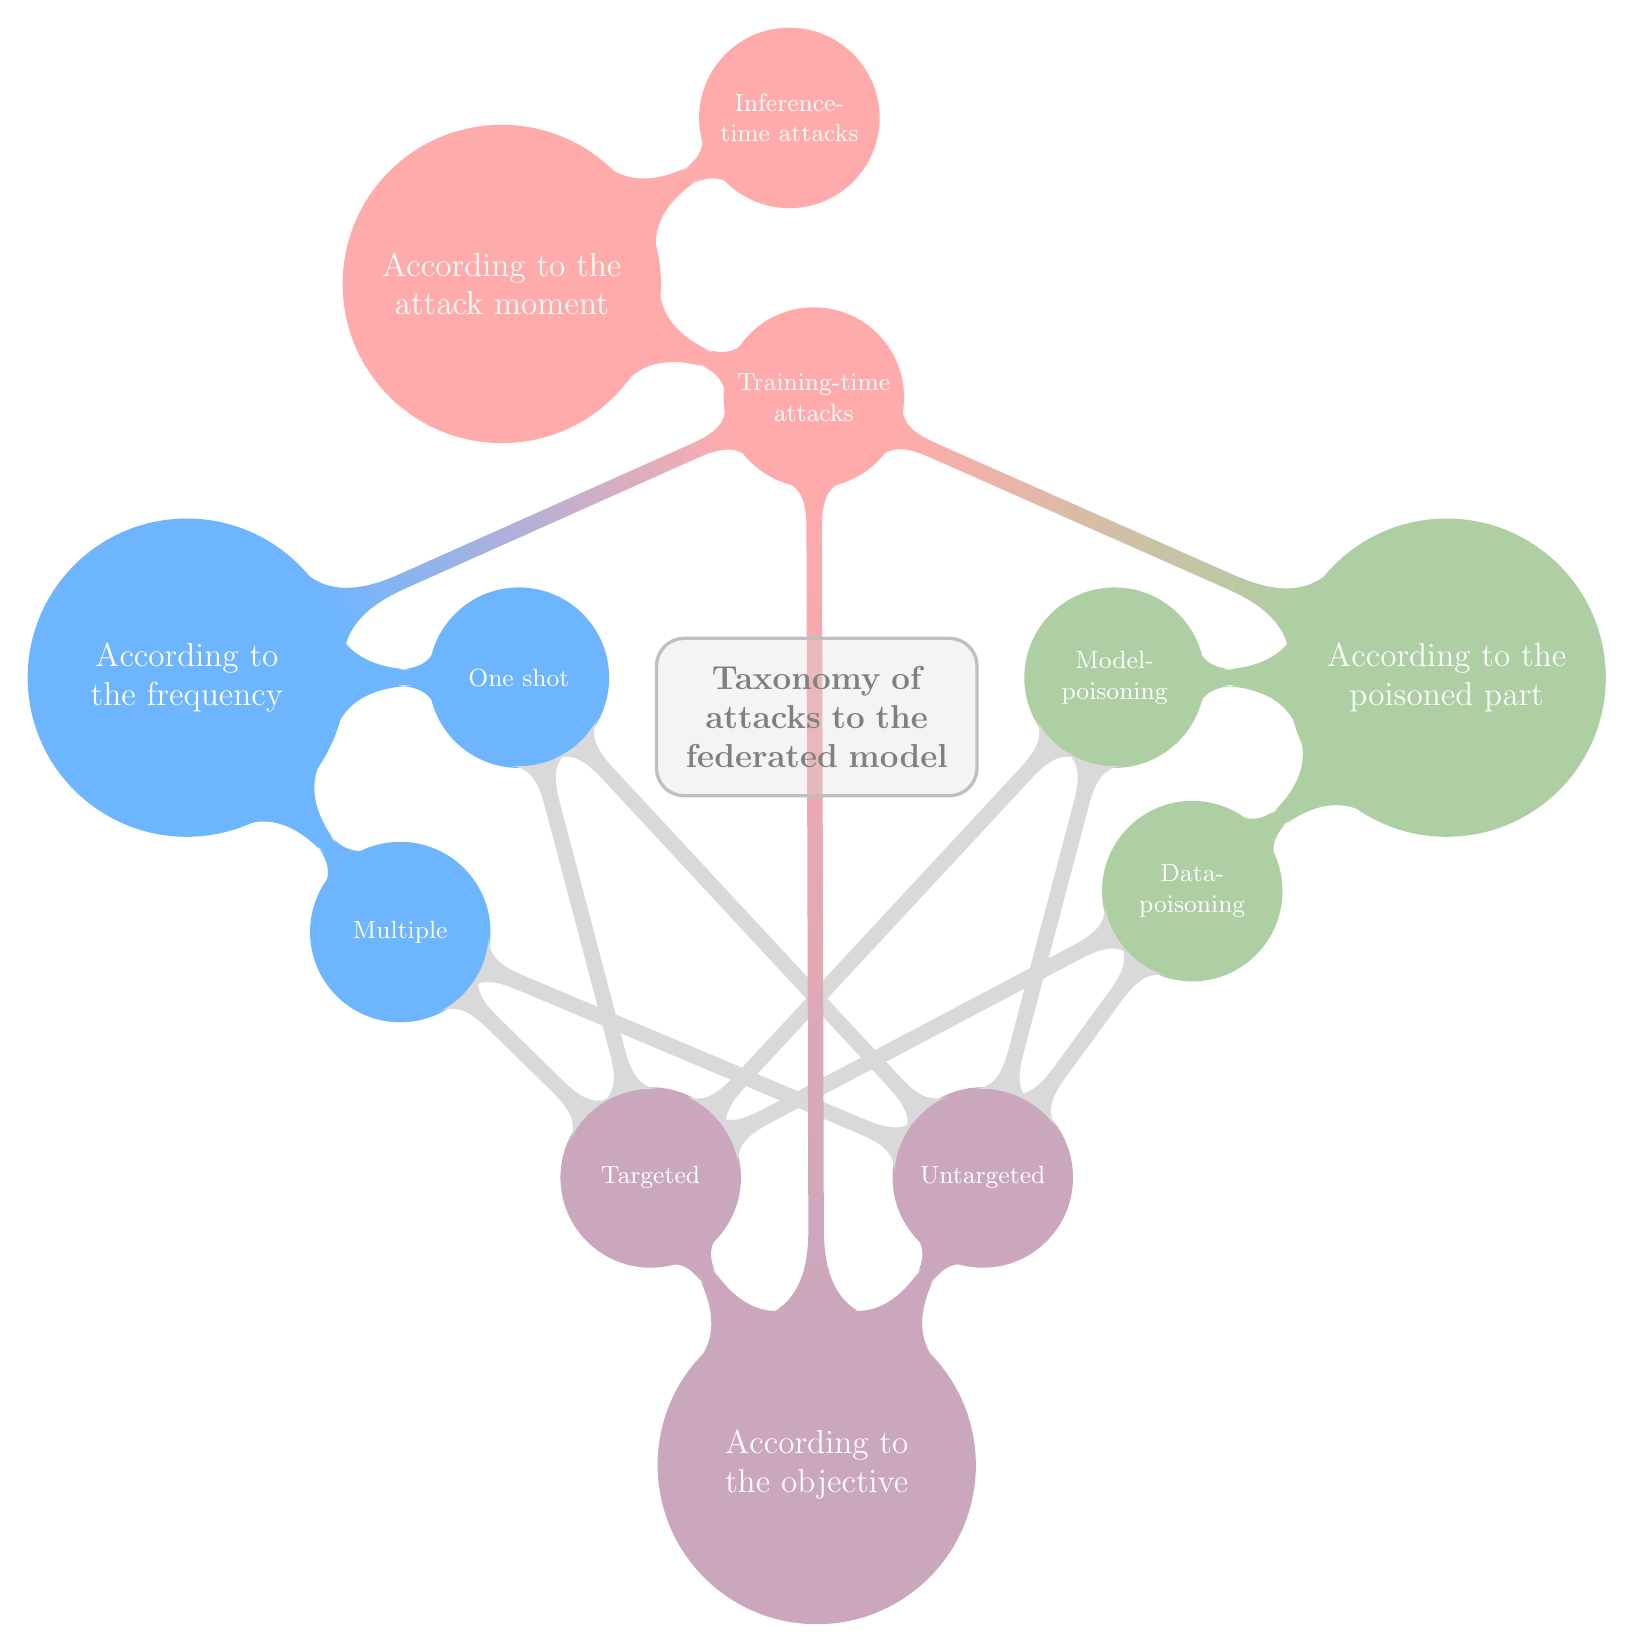
\begin{tikzpicture}[mindmap,
  level 1 concept/.append style={level distance=130,sibling angle=30},
  extra concept/.append style={color=morado_pastel!50,text=black}]

    \definecolor{rojo_pastel}{HTML}{FFABAB}
    \definecolor{azul_pastel}{HTML}{6EB5FF}
    \definecolor{verde_pastel}{HTML}{ADCFA3}
    \definecolor{morado_pastel}{HTML}{CAA7BD}

    

  % Applied area: computer science and its subfields

  \begin{scope}[mindmap, concept color=rojo_pastel, text=white]
    \node [concept] at (-4, 3) {According to the attack moment}
      child [grow=30, level distance=120] {node [concept] (test) {Inference-time attacks}}
      child [grow=-20, level distance=120] {node [concept] (training) {Training-time attacks}};
  \end{scope}

  % Applied area: theoretical physics and its subfields

  \begin{scope}[mindmap, concept color=azul_pastel,text=white]
    \node [concept] (frequency) at (-8,-2) {According to the frequency}
      child [grow=-50, level distance=120]
        {node [concept] (mul) {Multiple}}
      child [grow=0, level distance=120] 
        {node [concept] (one) {One shot}};
  \end{scope}
  
  
    \begin{scope}[mindmap, concept color=morado_pastel,text=white]
    \node [concept] (objective) at (0,-12) {According to the objective}
      child [grow=120, level distance=120]
        {node [concept] (tar) {Targeted}}
      child [grow=60, level distance=120] 
        {node [concept] (untar) {Untargeted}};
  \end{scope}

    \begin{scope}[mindmap, concept color=verde_pastel,text=white]
    \node [concept] (part) at (8,-2) {According to the poisoned part}
      child [grow=220, level distance=120]
        {node [concept] (data) {Data-poisoning}}
      child [grow=180, level distance=120] 
        {node [concept] (model) {Model-poisoning}};
  \end{scope}



  % Connections of researchers to applied subfields


    \path (one) to[circle connection bar switch color=from (black!15) to (black!15)] (tar);
    \path (one) to[circle connection bar switch color=from (black!15) to (black!15)] (untar);
    \path (mul) to[circle connection bar switch color=from (black!15) to (black!15)] (tar);
    \path (mul) to[circle connection bar switch color=from (black!15) to (black!15)] (untar);
    \path (data) to[circle connection bar switch color=from (black!15) to (black!15)] (tar);
    \path (data) to[circle connection bar switch color=from (black!15) to (black!15)] (untar);
    \path (model) to[circle connection bar switch color=from (black!15) to (black!15)] (tar);
    \path (model) to[circle connection bar switch color=from (black!15) to (black!15)] (untar);

    
    \path (training) to[circle connection bar switch color=from (rojo_pastel) to (azul_pastel)] (frequency);
    \path (training) to[circle connection bar switch color=from (rojo_pastel) to (morado_pastel)] (objective);
    \path (training) to[circle connection bar switch color=from (rojo_pastel) to (verde_pastel)] (part);
    
     \node[rectangle, draw, fill=black!15, fill opacity=0.3,draw = lightgray, rounded corners = 10pt, text opacity = 1, text = gray, text width=4cm, minimum height = 2cm] (r) at (0,-2.5) {\large \textbf{Taxonomy of attacks to the federated model}};


\end{tikzpicture}}
\end{center}
